%-----------------------------------------------------------------------------
%
%               Template for sigplanconf LaTeX Class
%
% Name:         sigplanconf-template.tex
%
% Purpose:      A template for sigplanconf.cls, which is a LaTeX 2e class
%               file for SIGPLAN conference proceedings.
%
% Guide:        Refer to "Author's Guide to the ACM SIGPLAN Class,"
%               sigplanconf-guide.pdf
%
% Author:       Paul C. Anagnostopoulos
%               Windfall Software
%               978 371-2316
%               paul@windfall.com
%
% Created:      15 February 2005
%
%-----------------------------------------------------------------------------

\documentclass[10pt,numbers]{sigplanconf}

% The following \documentclass options may be useful:

% preprint      Remove this option only once the paper is in final form.
% 10pt          To set in 10-point type instead of 9-point.
% 11pt          To set in 11-point type instead of 9-point.
% numbers       To obtain numeric citation style instead of author/year.

\usepackage{amsmath}
\newcommand{\cL}{{\cal L}}

\usepackage[utf8]{inputenc}
\usepackage[T1]{fontenc}
\usepackage{microtype}

\usepackage{tabularx, booktabs, array, dcolumn}
\usepackage{dsfont}
\usepackage{listings}
%\usepackage{caption}
\usepackage{xcolor}
\usepackage{graphicx}
\usepackage{float}
%\usepackage[sectionbib]{natbib}
\renewcommand{\bibsection}{\section*{REFERENCES}}

%\newcolumntype{Z}{>{\raggedright}X}
%\setlength{\textfloatsep}{5pt plus 1.0pt minus 1.0pt}
%\setlength{\dbltextfloatsep}{5pt plus 1.0pt minus 1.0pt}
%\setlength{\floatsep}{1pt plus 1.0pt minus 2.0pt}
%\setlength{\dblfloatsep}{1pt plus 1.0pt minus 2.0pt}

\definecolor{commentsColor}{rgb}{0.497495, 0.497587, 0.497464}
\definecolor{keywordsColor}{rgb}{0.000000, 0.000000, 0.635294}
\definecolor{stringColor}{rgb}{0.558215, 0.000000, 0.135316}

\lstset{%
language=C++,
basicstyle=\fontsize{9pt}{10pt}\ttfamily,
numbers=left,
numbersep=5pt,
xleftmargin=14pt,
keepspaces=true,
frame=tb,
framexleftmargin=14pt,
breaklines=true,                 % sets automatic line breaking
captionpos=b,                    % sets the caption-position to bottom
commentstyle=\color{commentsColor}\textit,    % comment style
escapeinside={\%*}{*)},     % if you want to add LaTeX within your code
numberstyle=\tiny\color{commentsColor},
columns=flexible,
showtabs=false,
stringstyle=\color{stringColor},
tabsize=2,
keywords={for, parallel, update, split, rfactor, compute_root, where, compute_at, vectorize},
keywordstyle=\color{keywordsColor}\bfseries,
belowskip=3pt
}

\newcommand{\code}[1]{\texttt{#1}}

\newcolumntype{d}{D{.}{.}{2.3}}
\newcolumntype{C}{>{\centering}m}

\clubpenalty = 10000
\widowpenalty = 10000
\displaywidowpenalty = 10000

\usepackage{flushend}
\usepackage{balance}

\begin{document}

\makeatletter
\def\@copyrightspace{\relax}
\makeatother

\special{papersize=8.5in,11in}
\setlength{\pdfpageheight}{\paperheight}
\setlength{\pdfpagewidth}{\paperwidth}

\conferenceinfo{CONF 'yy}{Month d--d, 20yy, City, ST, Country}
\copyrightyear{20yy}
\copyrightdata{978-1-nnnn-nnnn-n/yy/mm}
\copyrightdoi{nnnnnnn.nnnnnnn}

% Uncomment the publication rights you want to use.
%\publicationrights{transferred}
%\publicationrights{licensed}     % this is the default
%\publicationrights{author-pays}

\titlebanner{banner above paper title}        % These are ignored unless
\preprintfooter{short description of paper}   % 'preprint' option specified.

\title{Parallel Associative Reductions in Halide}

% 1st. author
\authorinfo{Patricia Suriana}
           {Google, USA}
           {psuriana@google.com}
% 2nd. author
\authorinfo{Andrew Adams}
           {Google, USA}
           {abadams@google.com}
% 3rd. author
\authorinfo{Shoaib Kamil}
           {Adobe, USA}
           {kamil@adobe.com}

\maketitle
\begin{abstract}

  Halide is a domain-specific language for fast image processing that separates pipelines into the \emph{algorithm}, which defines \emph{what} values are computed, and the \emph{schedule}, which defines \emph{how} they are computed. Changes to the schedule are guaranteed to not change the results. While Halide supports parallelizing and vectorizing naturally data-parallel operations, it does not support the same scheduling for reductions. Instead, the programmer must create data parallelism by manually factoring reductions into multiple stages. This manipulation of the \emph{algorithm} can introduce bugs, impairs readability and portability, and makes it impossible for automatic scheduling methods to parallelize reductions.

  We describe a new Halide scheduling primitive \code{rfactor} which moves this factoring transformation into the \emph{schedule}, as well as a novel synthesis-based technique that takes serial Halide reductions and synthesizes an equivalent binary associative reduction operator and its identity. This enables us to automatically replace the original pipeline stage with a pair of stages which first compute partial results over slices of the reduction domain, and then combine them. Our technique permits parallelization and vectorization of Halide algorithms which previously required manipulating both the algorithm and schedule.

\end{abstract}

%\category{CR-number}{subcategory}{third-level}

% general terms are not compulsory anymore,
% you may leave them out
%\terms
%term1, term2

%\keywords
%keyword1, keyword2

\section{Introduction}
\label{introduction}
Halide \cite{Ragan-Kelley:2013:HLC:2491956.2462176} is important, provides separation of algorithm and schedule. Ability to try various schedules with guaranteed correctness and consistency: different schedules are guaranteed to produce the same output as long they define the same computation. \\

One important class of problems: associative reduction. This can be as simple as single-dimensional sum or some complex multidimensional associative ops (see Figure 1). One way to optimize performance in associative reduction: split into smaller chunks of works, compute them separately, and merge the partial result. Associative property allows such optimization. \\

Figure:

\begin{lstlisting}[
caption = {make the case that they're both associative reductions, but it's not obvious what the binary operator is from the code for the second one}]
Summation (easy example)

Func out;
out() = 0;
RDom r(0, input.width());
out() = out() + input(r.x);

The complex number with the greatest magnitude, 
and its location (hard example)

Func out;
out() = {0, 0, 0};
RDom r(0, input.width(), 0, input.height());
Expr real = input(r.x, r.y)[0];
Expr imag = input(r.x, r.y)[1];
Expr mag = real * real + imag * imag;
Expr best_mag = out()[0] * out()[0] + out()[1] * out()[1];
Expr c = mag > best_mag;
out() = {select(c, real, out()[0]),
         select(c, imag, out()[1]),
         select(c, r.x, out()[2]),
         select(c, r.y, out()[3])};
\end{lstlisting}

However, Halide did not support parallel or *vectorized* reductions till now without changing algorithm (which fails to deliver core promise of language in which schedule and algorithm should be separate and not affect each other). We present a Halide scheduling primitive (DAG transformation) that creates a new data parallelizable/vectorizable axis out of a reduction. \\

rfactor splits an update (**associative update**) into an intermediate which computes the partial results and a new update definition which merges the partial results -> creates separate copies of the reduction dimension which exposes a new data parallelism (parallelizable + vectorizable), and a second stage that combines those partial results. Combined with other Halide scheduling directives, such as split, this allows Halide to represent a broader class of schedules, including parallel associative reduction. 

<Insert some code snippet of pipeline produced by rfactor, including performance numbers for it -> serial, hand-rolled, using rfactor> \\

Other benefits: code reduction, supports purity/separation of algorithm and schedule, and portability, which is especially important for auto-scheduling \cite{Mullapudi:2016:ASH:2897824.2925952}. \\


%\vspace*{-5pt}
\section{Background \& Related Work}
\label{background}
Programmers define the \emph{algorithm} in Halide through a Halide \emph{function}, which consists of sequence of stages; these stages are the unit on which scheduling occurs. By default, each stage represents a perfectly-nested loop nest in which a single value of the \emph{function} is computed and stored in the innermost loop per iteration. Stages after the first are called \emph{update} stages, and are allowed to recursively refer to the function. Some of the loops are data parallel and are constrained to be race-condition free by syntactic restrictions. These data-parallel loops iterate over variables called \code{Var}s. The bounds of these loops are inferred by Halide using interval arithmetic.  Other loops may have user-specified bounds and a user-specified nesting order, and fewer syntactic restrictions on their use. These are known as \code{RVar}s (for reduction \code{Vars}), which together define a reduction domain or \code{RDom}. \code{RVar}s are used to express reductions, scattering, scans, etc. Each of these loop types, defined by \code{Var}s and \code{RVar}s, can be manipulated in various ways through Halide scheduling primitives: they can be tiled, unrolled, mutually interchanged, etc., provided that the nesting order of \code{RVar}s is respected. 

While \code{Var}s are safe to parallelize or vectorize by construction -- \code{Var}s represents the naturally data-parallel axes of an \emph{algorithm} -- \code{RVar}s can be parallelized or vectorized if and only if Halide can prove that no race condition exists. This makes parallelizing or vectorizing stages that use only \code{RVar}s difficult. For example, consider the two-dimensional convolutional blur kernel shown in Listing~\ref{lst:blur_loopness}, which is easily parallelizable across \code{Var} $x$ and $y$. The histogram of an image (see Listing~\ref{lst:histogram_loopness}), on the other hand, is harder to parallelize since its update stage only involves \code{RVar}s. In order to parallelize a reduction like histogram, one needs to be able to factorize it into slices that have no dependencies on each other.

Although much prior work has explored automatic generation of parallel associative reductions from a serial reduction, most work assumes an explicit associative binary reduction operator is given, which is not applicable to Halide. Since Halide does not support reduction using a binary operator as a first-class primitive, reductions in Halide are implemented through usage of non-data-parallel \code{RVar}s. For Halide to support parallel reductions, it needs to be able to deduce an equivalent binary associative reduction operator and its identity from a serial reduction expressed as an imperative Halide \emph{update}. 

Prior work by Morita et al.~\cite{Morita:2007:AIG:1250734.1250752} introduced automatic generations of divide-and-conquer parallel programs framework based on the third homomorphism theorem and derivation of weak-right inverse. However, it requires programmers to specify the leftwards and rightwards forms of the sequential function which may not be obvious to derive. Teo et al.~\cite{Teo:1997:DEP:266670.266697} proposed a method to synthesize parallel divide-and-conquer
programs from a recurrence function (which is similar in form to a Halide serial reduction) through induction. They first derive two equivalent pre-parallel forms of the recurrence function by applying some generalization rules and deduce the intermediate and merge reduction functions through induction on those two pre-parallel forms. Although it can be applied to solve some complex recurrences, such as reduction of complex multiplication, the technique requires long derivation time and is unable to deal with reductions like \code{argmin}, which require non-trivial re-ordering of the chain of conditionals during the induction steps. 

Recent work has applied program synthesis, which automatically discovers executable code based on user intent derived from examples or other constraints, to generate parallel programs. Smith et al.~\cite{Smith:2016:MPS:2908080.2908102} used program synthesis to automatically generate MapReduce-style distributed programs from input-output examples. \textsc{Sketch}~\cite{Solar-Lezama:2008:PSS:1714168} and \textsc{Rosette}~\cite{Torlak:2013:GSL:2509578.2509586} are two solver-aided programming languages with support for program synthesis.  MSL~\cite{Xu:2014:MSE:2683593.2683628} is a synthesis-based language for distributed implementations that can derive many details of the distributed implementation from serial specifications.  We discuss \textsc{Sketch} and \textsc{Rosette} in Section~\ref{synthesize}.

Superoptimization~\cite{Granlund:1992:EBU:143095.143146, Massalin:1987:SLS:36206.36194} searches for the shortest or most optimized way to compute a branch-free sequence of instructions, by exhaustively searching over a space of possible programs. These rewrites can then be turned into peephole optimizations in compilers. More recent work has used stochastic search~\cite{Phothilimthana:2016:SUS:2872362.2872387, Schkufza:2013:SS:2490301.2451150} and program synthesis~\cite{Lopes:2015:PCP:2737924.2737965} to find replacements for larger sequences of instructions.
In this work, we find equivalent replacements for a Halide reduction through a combination of enumeration and synthesis; in addition, though our domain is more restricted, we search for larger replacements than most superoptimizers.

\begin{lstlisting}[caption={Convolution blur kernel is easily parallelizable across \code{Var} $x$ adn $y$.}, label={lst:blur_loopness}]
// First stage
for y in range(input.height()):
  for x in range(input.width()):
    blur[x][y] = 0
// Update stage
parallel for y in range(input.height()):
  parallel for x in range(input.width()):
    for ry in range(kernel.height()):
      for rx in range(kernel.width()):    
        blur[x][y] += 
          kernel[rx][ry]*input[x+rx-1][y+ry-1] 
\end{lstlisting}

\begin{lstlisting}[caption={Histogram of an image is hard to parallelize since its update stage does not involve \code{RVar}s.\textbf{SK: it doesn't involve Rvars?}}, label={lst:histogram_loopness}]
// Serial version
// First stage
for x in range(256):
  hist[x] = 0
// Update stage
for ry in range(input.height()):
  for rx in range(input.width()):
    hist[clamp(int(input[rx][ry]), 0, 255)] += 1
\end{lstlisting}


\section{The \code{rfactor} Transformation}
\label{assoc_red}
\subsection{Reductions in Halide}

Serial reductions in Halide (e.g. summation over an array, histogram, etc.) are implemented using \code{RVar}s or \code{RDom}s. An \code{RVar} is an implicit serial loop, and an \code{RDom} is an ordered list of \code{RVar}s specifying a serial loop nest. Since \code{RVar}s are not trivially parallelizable or vectorizable, a programmer must manually \emph{factor} a reduction into an \emph{intermediate} function that performs reduction over distinct slices of the domain, and a \emph{merge} function that combines those partial results.

This manual manipulation is tedious and error-prone, especially when the reduction domain is non-rectangular (see Listing \ref{lst:circular_max_1}). To further complicate matters, it is hard to infer what binary reduction operator is equivalent to a Halide update definition, and even then, many binary operators are not obviously associative (e.g. $x + y + 7xy$ is in fact associative). We will defer these issues to section \ref{synthesize}, and for now assume that given a Halide update definition we can deduce the equivalent associative binary operator and its identity. Note that we do not require the binary operators to be commutative.

\subsection{The \code{rfactor} Transformation}

To remove the burden of \emph{factoring} a reduction from the programmer, we introduce a new scheduling primitive called \code{rfactor}. This splits a reduction into pair of reductions, which we will call the \emph{intermediate} stage and the \emph{merge} stage. \code{rfactor} takes as input a list of \code{<RVar, Var>} pairs. \code{RVar}s not in the list are removed from the \emph{merge} stage and lifted to the \emph{intermediate} stage. The remaining \code{RVar}s become \code{Var}s in the \emph{intermediate} stage, which allows them to be parallelized or vectorized. See Figure \ref{fig:rfactor} for a simple example. The listings below demonstrate more complex usage.

 Note that we limit the scope of \code{rfactor} to reductions where the \emph{intermediate} and \emph{merge} stages have the same equivalent binary associative reduction operator. For instance, if the equivalent binary associative reduction operator of the \emph{intermediate} stage is \code{min(x, y)}, then that of the \emph{merge} stage must also be \code{min(x, y)}. Another restriction is that the binary associative operator must have an identity, as it is used to initialize the \emph{intermediate} stage. Not all associative binary operators have identities (e.g. $2xy$, where $x, y \in \mathds{Z}$).

\begin{lstlisting}[caption={Computing the histogram of a two-dimensional image in Halide. The RDom defines an implicit loop nest over \code{r.x} and \code{r.y}. Halide will not permit either of these loops to be parallelized, as that would introduce a race condition on the += operation.}, label={lst:histogram_rfactor_1}]
// Algorithm
Func hist;
Var i;
hist(i) = 0;
RDom r(0, input.width(), 0, input.height());
hist(input(r.x, r.y)) += 1;

// Schedule
hist.compute_root();
\end{lstlisting}

\begin{lstlisting}[caption={A manually-factored histogram. The programmer has introduced an intermediate function that computes the histogram over each row of the input. This intermediate is data-parallel over y, and so it can be parallelized. The original function \code{hist} now merely sums these partial histograms. It is data-parallel over histogram buckets, and the programmer has vectorized it.}, label={lst:histogram_rfactor_2}]
// Algorithm
Func intm;
Var i, y;
intm(i, y) = 0;
RDom rx(0, input.width());
intm(input(rx, y)) += 1;

Func hist;
hist(i) = 0;
RDom ry(0, input.height());
hist(i) += intm(i, ry);

// Schedule
intm.compute_root().update().parallel(y);
hist.compute_root().update().vectorize(i, 4);
\end{lstlisting}

\begin{lstlisting}[caption={Using \code{rfactor}, the programmer can produce the same machine code as in \ref{lst:histogram_rfactor_2}, using the simpler algorithm in \ref{lst:histogram_rfactor_1}. While the schedule is more complex, recall that it is only the five lines of algorithm that determines correctness. The programmer was able to transform the code to exploit parallelism without risking introducing a correctness bug.}, label={lst:histogram_rfactor_3}]
// Algorithm
Func hist;
Var i;
hist(i) = 0;
RDom r(0, input.width(), 0, input.height());
hist(input(r.x, r.y)) += 1;

// Schedule
Var y;
hist.compute_root()
Func intm = hist.update().rfactor(r.y, y);
intm.compute_root().update().parallel(y);
hist.update().vectorize(i, 4);
\end{lstlisting}

\begin{lstlisting}[caption={Computing the maximum over a circular domain. Reduction domains need not be rectangular. In this case we use \code{RDom::where} to restrict it to the points that lie within a circle of radius 10.}, label={lst:circular_max_1}]
// Algorithm
Func max_val;
max_val() = 0;
RDom r(0, input.width(), 0, input.height());
r.where(r.x*r.x + r.y*r.y <= 100);
max_val() = max(max_val(), input(r.x, r.y));

// Schedule
max_val.compute_root();
\end{lstlisting}

\begin{lstlisting}[caption={Manually factoring this reduction requires also manipulating the predicate associated with the RDom. The identity for \code{max} is the minimum value of the type in question.}, label={lst:circular_max_2}]
// Algorithm
Func intm;
Var y;
intm(y) = input.type().min();
RDom rx(0, input.width());
rx.where(rx*rx + y*y <= 100);
intm(y) = max(intm(y), input(rx, y));

Func max_val;
max_val() = 0;
RDom ry(0, input.height());
max_val() = max(max_val(), intm(ry));

// Schedule
intm.compute_root();
    .update().parallel(y);
max_val.compute_root();
\end{lstlisting}

\begin{lstlisting}[caption={Using \code{rfactor} in the schedule can produce the same machine code from the simpler form of the algorithm.}]
// Algorithm
Func max_val;
max_val() = 0;
RDom r(0, input.width(), 0, input.height());
r.where(r.x*r.x + r.y*r.y <= 100);
max_val() = max(max_val(), input(r.x, r.y));

// Schedule
Var y;
max_val.compute_root();
Func intm = max_val.update().rfactor(r.y, y);
intm.compute_root();
    .update().parallel(y);
\end{lstlisting}




\section{Synthesizing Associative Binary Operators}
\label{synthesize}
% Overview of section
In the previous section, we described how \code{rfactor} transforms a Halide reduction to expose new data parallelism. Doing so requires synthezising the associative binary operator equivalent to the Halide \emph{update} definition being factored. In this section we describe how we do this synthesis.

% Set up problem, LUT solution
In some cases generating the equivalent associative operator from an update definition is trivial (e.g.\ summation). In other cases it is not, especially when the function reduces onto multiple values (see the examples in Figure~\ref{fig:subgraphs}). The \emph{inverse} problem is easier: Given an associative binary operator, it is straightforward to generate the Halide update definition that implements reduction by it. Therefore, if there were a \emph{small} finite set of associative binary operators, we could simply attempt to match the update definition being factored against each of them in turn. Halide already includes facilities for doing regex-like matching of expressions against patterns with wildcards. Unfortunately, there are more meaningful associative binary operators than could reasonably be thought of ahead of time by a compiler author.

% Full synthesis solution
An alternative approach is to use program synthesis techniques~\cite{Solar-Lezama:2008:PSS:1714168, Torlak:2013:GSL:2509578.2509586} to synthesize the corresponding associative reduction at compile-time when the call to \code{rfactor} is made. This is intractably slow, and can increase compile times of Halide pipelines from seconds to hours.

% Our solution
We use a hybrid of the two approaches, amplified with a strategy for decomposing each synthesis problem into several simpler problems. The overall strategy is shown in Figure~\ref{fig:system}.  Offline, we generate a large finite table of one- and two-dimensional \emph{elementary} associative binary operators and their identities. These are akin to primes -- they are the associative operators which cannot be decomposed into a combination of simpler associative binary operators. At compile-time, we decompose the given Halide update definition into a composition of simpler, lower-dimensional definitions in the same way, then search the table for the elementary operator corresponding to each. If consistent matches are found, we reassemble the results into a composite associative operator equivalent to the original update definition. In Section~\ref{subsec:generation} we describe how we generate the table, and in Section~\ref{subsec:decomposition} we describe the decomposition procedure.

\subsection{Generating Elementary Operators}
\label{subsec:generation}

We begin with an enumeration of all one- and two-dimensional tuples of expression trees in two tuple inputs $x$ and $y$. The operators used to form the inner nodes of the trees are Halide's IR nodes (\code{*}, \code{+}, \code{-}, \code{min}, \code{max}, \code{select}, \code{<}, etc). We can reject some classes of uninteresting expressions by excluding them from the enumeration altogether.

\begin{enumerate}
\item We only generate trees which use both $x$ and $y$.
\item During matching we canonicalize both the pattern and the input expression using the Halide simplifier and solver; thus, we can make the enumeration more tractable by only generating trees that are already in canonical form.  The canonicalization strategy moves all instances of a variable in an expression tree as far to the left and as far up the tree as possible. We canonicalize expressions to the following form: wherever possible, $x_i$ is to the left of $x_{i+1}$ and any $y_j$ is to the left of $y_{j+1}$. Constants are always on the right.
\item We generate trees using a single generic constant $k$, rather than generating trees containing all possible constants as leaves.
\item We do not generate trees that would be trivially simplified. For example, we do not generate subexpressions like $max(x_0, x_0)$.
\end{enumerate}

After generating a large set of candidate expressions in this manner, we then subject the expressions to a battery of tests so that only elementary associative operators remain. The tests are arranged in increasing order of expense, so that we can cheaply reject most expressions.

\begin{enumerate}
\item For an operator $f$, we construct the expressions $f(f(x, y), z)$ and $f(x, f(y, z))$, and substitute in 100 randomly-selected values for $x, y, z, k$. If the two expressions don't evaluate to the same thing, the expression is not associative and can be rejected.
\item We then reject operators which can be decomposed using the decomposition procedure in Subsection~\ref{subsec:decomposition}.
\item Finally, to \emph{prove} that the expression is associative, we use the Z3~\cite{DeMoura:2008:ZES:1792734.1792766} SMT solver to verify that $\forall x, y, z, k \;f(f(x, y), z) = f(x, f(y, z))$, where $k$ is the constant contained within the function $f$. If this proof succeeds, we then ask Z3 to solve $\forall x, k \;f(id, x) = x$ to synthesize the identity $id$.
\end{enumerate}

In the table of expressions that this produces, $x$ represents the partial result being reduced onto, and $y$ is a wildcard which could match any expression. When matching, $x$ must also appear on the left-hand-side of the update definition. $y$ may depend on the reduction domain coordinates, but may not depend on the partial results. The constant $k$, if it exists, may match anything which neither depends on the reduction domain coordinates nor the partial result. For example, the update definition which separately computes the sum-of-squares of the even and odd values of some input \code{in} could be written as:

\code{f(in(r)\&1) = f(in(r)\&1) + in(r)*in(r)}

This would match against the pattern $x = x + y$, where $x$ matches \code{f(in(r)\&1)}, and $y$ matches \code{in(r)*in(r)}.

We terminate the enumeration at trees with 8 leaves for the purposes of the experiments described in this work. Since some operations are associative in certain scalar types and not others, we generate different tables for each of Halide's scalar types.  This takes 1.5 days and generates around 9,000 elementary operators to match against per type\footnote{Due to deadline constraints, we only ran the enumeration for \code{uint32} and {int32} types, generating a total of 17,905 fragments.  We plan to run the enumeration for all additional elementary types supported by Halide.}. Many of the operators are simple operators written in a complex way: as we wish to catch all ways in which a programmer might write a reduction, we make no attempt to exclude these from the table. The first 10 elementary associative operators for signed 32-bit integers are shown in Listing~\ref{lst:top10}.

\begin{lstlisting}[caption={The first 10 elementary associative operators for 32-bit signed integers}, label={lst:top10}]
x + y
x * y
min(x, y)
max(x, y)
max(min(x, k), y)
min(max(x, k), y)
max(min(y, k), x)
min(max(y, k), x)
max(min(k - x, y), x)
min(max(k - x, y), x)
\end{lstlisting}

%As the list grows, operators become more and more esoteric. An example 8-leaf operator from the list for unsigned integers is TODO

As we only consider one- and two-dimensional expressions, there are meaningful primitive operators that we never discover. For example, we never generate quaternion multiplication, since it is an elementary associative operator in 4 tuple elements, where every expression tree has 8 leaf nodes. We must add any important higher-dimensional primitive operators to our table manually.

%Another limitation is that for each associative reduction, we have a single pattern for the update definition we expect to see, and so if the Halide simplifier and solver fail to canonicalize an update definition into that form, we will not recognize it. For example, consider the reduction which counts how many points in the reduction domain satisfy some predicate $P$. It may be written with the addition outermost:

%\code{f() = select(P(r), 1, 0) + f()}

%After canonicalization we recognize this as a sum reduction of the form \code{x = x + y}. One might also write it with the \code{select} outermost:

%\code{f() = select(P(r), f() + 1, f())},

%We do not recognize this as a sum reduction.

\begin{figure}[tb]
\centering
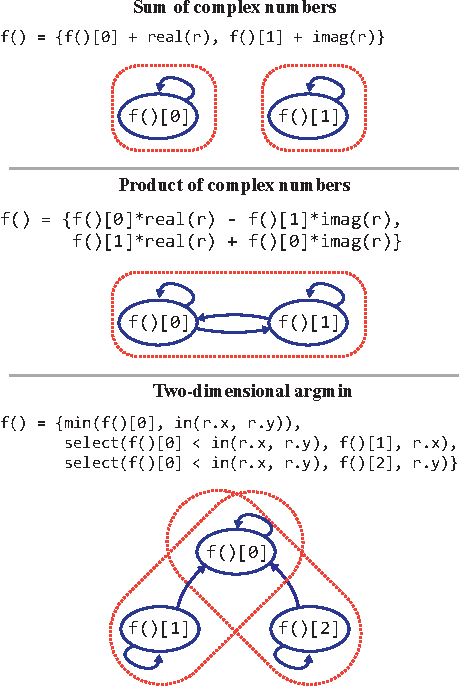
\includegraphics{subgraphs}
\caption{Dependency graphs of various multi-valued Halide \emph{update} definitions. Their subgraph decompositions are shown in red. To find the associative operator equivalent to a complex Halide update definition, we first decompose it into subgraphs, then search for each subgraph in our precomputed table of elementary operators, then recompose the results into a single multi-valued associative operator.}
\label{fig:subgraphs}
\end{figure}

\subsection{Subgraph Decomposition}
\label{subsec:decomposition}

To describe how we decompose reductions into elementary operators, we must first discuss how one might \emph{compose} elementary reductions. The simplest way to compose two reductions into a higher-dimensional reduction is to compute them at the same time, independently. This means that reductions that are a concatenation of smaller independent associative reductions are also associative. For example, the tuple computation:

\code{f() = \{f()[0] + in(r), f()[1] * in(r)\}}

is associative, because it is a composition of the following two associative reductions:

\code{f0() = f0() + in(r)}

\code{f1() = f1() * in(r)}

Secondly, if we have an associative operator in which two tuple elements compute the same value, we can deduplicate it, reducing the dimensionality by one. The result is still associative. Therefore, we can prove a reduction is associative by duplicating one of the elements to break a dependency and then applying the rule above. Consider the case of two-dimensional \code{argmin}:

\begin{lstlisting}
f() = {
  min(f()[0], in(r.x, r.y)),
  select(f()[0] < in(r.x, r.y), f()[1], r.x),
  select(f()[0] < in(r.x, r.y), f()[2], r.y)}
\end{lstlisting}

The three tuple elements are the minimum value, and its $x$ and $y$ coordinate. All three tuple elements depend on the minimum value \code{f()[0]}, so we can't decompose this into independent reductions immediately. Let's duplicate the first tuple element to break the dependency:

\begin{lstlisting}
f() = {
  min(f()[0], in(r.x, r.y)),
  select(f()[0] < in(r.x, r.y), f()[1], r.x),
  min(f()[2], in(r.x, r.y)),
  select(f()[2] < in(r.x, r.y), f()[3], r.y)}
\end{lstlisting}

There are now no dependencies between the first two elements and the last two. This is a simple concatenation of two single-variable \code{argmin} operations. Single-variable \code{argmin} uses two tuple elements, and is present in our table of primitive operators, so we recognize two-dimensional \code{argmin} as associative via its decomposition into two one-dimensional \code{argmin} reductions.

In general we consider the directed graph of dependencies between tuple elements. There is a vertex per tuple element, and an edge from vertex $i$ to vertex $j$ whenever the definition of tuple element $i$ refers to tuple element $j$. If we repeatedly duplicate vertices (tuple elements) to break dependencies, in the limit the graph has one connected component per original tuple element, and that component is the subgraph containing the vertices reachable from that tuple element. If each such subgraph is an associative reduction, then the original reduction is associative. See Figure~\ref{fig:subgraphs} for several examples.

%The general way to apply these two rules to decompose an arbitrary reduction into its components is to construct the directed graph $G$ of dependencies between tuple elements. There is a vertex $N_i$ for each tuple element $i$, and there is an edge from $N_i$ to $N_j$ whenever the value of tuple element $i$ depends on tuple element $j$. The two rules above can then be stated as:

%\begin{enumerate}
%\item If every connected component of $G$ is an associative reduction, then $G$ is an associative reduction.
%\item If we duplicate one of the nodes of $G$, partitioning its incoming edges arbitrarily between the two copies, then the resulting graph is associative iff $G$ is associative, as they compute the same thing.
%\end{enumerate}

% This is a shitty ``proof''
%Let the subgraph $S_i$ be all vertices and edges reachable from $N_i$. We can make a copy of $S_i$ as its own connnected component set apart from the rest of $G$ by the following procedure: Initialize $S_i$ to contain only a duplicate of $N_i$, with no incoming edges. Then repeatedly consider all edges that leave $S_i$, and make duplicates of the vertices they point to, where edges from vertices within $S_i$ point to the duplicate, and edges from vertices not in $S_i$ point to the original. This procedure terminates when $S_i$ contains all vertices reachable from $N_i$. At that point, there are no edges between $S_i$ and the rest of $G$, so it is its own connected component. Once we construct each such $S_i$, we can discard $G$, as everything it computes is also computed by one of the disconnected subgraphs. Similarly, we can discard subgraphs which are completely contained by some other subgraph. Therefore, if every subgraph $S_i$ not contained within some other subgraph is an associative reduction, then $G$ is an associative reduction. For examples of these graphs and their subgraphs for several reductions see Figure \ref{fig:subgraph}.

% Merging results of decomposition
After finding the associative operator equivalent to each subgraph separately, we need to combine the results into a single multi-valued associative operator equivalent to the entire update definition. If all the subgraphs are associative and have identities, we need to ensure that for each tuple element appearing in multiple subgraphs, the binary associative operators deduced via each subgraph are all the same in that tuple element. If they are consistent, we have succeeded in finding an equivalent multi-valued associative operator for the update definition.

In some cases, this procedure over-partitions the graph. We are searching for an associative operator in $x$ and $y$. Only the $x$ is apparent from the Halide update definition -- it is the term that also appears on the left-hand-side. If we decompose based on cross-dependencies within $x$ alone we will miss dependencies between tuple elements that exist only in $y$. Consider 2x2 matrix multiplication written as a four-dimensional reduction:

\begin{lstlisting}
f() = {f()[0] * in(r)[0]) + f()[1] * in(r)[2]),
       f()[0] * in(r)[1]) + f()[1] * in(r)[3]),
       f()[2] * in(r)[0]) + f()[3] * in(r)[2]),
       f()[2] * in(r)[1]) + f()[3] * in(r)[3])}
\end{lstlisting}

Decomposition based on $x$ alone (i.e. \code{f()[i]}) results in 2 subgraphs: one containing the 1st and 2nd tuple elements and one containing the 3rd and 4th tuple elements. Including $y$ (i.e. \code{in(r)[i]}) tells us that the two subgraphs are indeed connected. Therefore, if we fail to find a match for the initial subgraphs (the ones decomposed based on $x$ only), we need to consider other possible grouping of those initial subgraphs. The total number of possible grouping is the Bell number of the initial number of subgraphs. However, we only need to consider grouping expressions which share a common subexpression, and we do not need to consider groups of size greater than the maximum tuple size in our precomputed table. If we do not find a matching associative operator under all possible groupings of the initial subgraphs, we terminate and return an error.

\begin{figure}[tb]
\centering
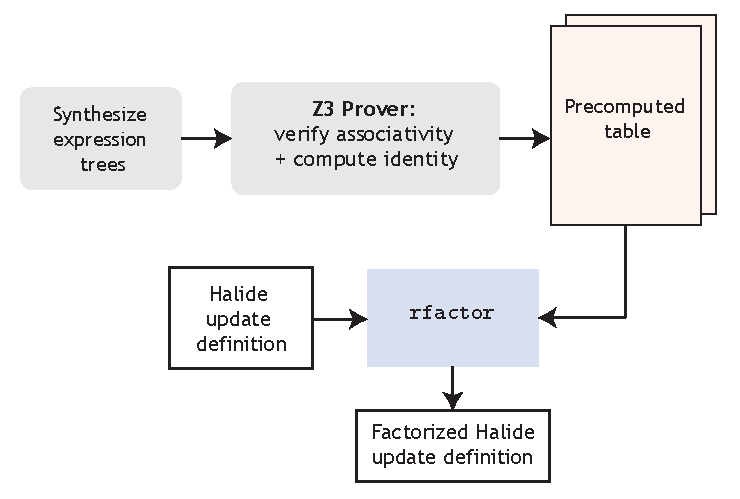
\includegraphics[width=3.2in]{system}
\caption{To factor a reduction written as a Halide update definition, we must first synthesize the equivalent associative binary operator. We generate a large table of elementary associative operators offline by enumerating all non-trivial expression trees and filtering out the ones that are not associative operators. At compile-time, we then decompose the given update definition into simpler definitions and match each against the table. Combining the results gives us the equivalent associative binary operator, which we can use to generate the factored form of the reduction}
\label{fig:system}
\end{figure}


\section{Evaluation}
\label{evaluation}
Performance results using rfactor (overall speedup): 2D argmin, complex multiplication, 2D histogram, dot product, matrix multiply. \\

Synthetic functions (also to show limitations): approximating 128-bit add with 2 64-bit integers -> z3 cannot prove that it is associative, although the max/min forms are provable with z3. \\

Limitations: we need an identity, symmetric intermediate and merge functions: they should be of the same form, constrained by the look-up table (we can only match to whatever are in the table -> whatever z3 can prove to be associative). Some associative ops (e.g. 4x4 matrix multiply) are just expensive to generate. Technically it's doable, provided we limit the ops to addition and multiplication and restricting the variables involved in the expr to be unique (no repeats) during lookup table generation. \\

Real-world stuff: same code that can be simplified when using rfactor \\

Performance of generation/search/synthesis. <TODO: Not sure what this is about? time taken when doing the matching? how many associative operations can be generated within some hours? > \\

Case study of importance of "code reduction"? <TODO: Not sure what this is about? > \\ 

\section{Conclusion}
\label{conclusion}
In this paper, we have presented a new Halide scheduling primitive called \code{rfactor}, which moves reduction factorization into the \emph{schedule}, while maintaining Halide's consistency guarantees. We have also introduced a novel synthesis-based technique that takes serial Halide reductions and synthesizes an equivalent binary associative reduction operator and its identity. These enable us to automatically decompose a reduction pipeline stage into a pair of stages: \emph{intermediate} stage that first computes partial results over slices of the reduction domain, and \emph{merge} stage that combines them. This, in turn, allows parallelization and vectorization of Halide algorithms which previously required manipulating both the algorithm and schedule. In addition to moving the burden of factoring a reduction from the programmer, \code{rfactor} also improves code readability and portability and further separates the \emph{algorithm} from its \emph{schedule} which enables automatic schedule generation tools to parallelize reductions. 

Although our framework is able to handle a broad range of reductions, there are several limitations. First, we constrain \code{rfactor} to handle only reductions where the \emph{intermediate} and \emph{merge} stages have the same equivalent binary associative reduction operator. The binary associative operator must also have an identity that is used to initialize the \emph{intermediate} stage. As a consequence, we are unable to handle some reduction operator such as \code{f() = f() -  g(r.x)} which in theory is parallelizable provided we use ``$-$'' for the \emph{intermediate} stage and ``$+$'' for the \emph{merge} stage. The types of expressions we can handle are also constrained by the pre-computed look-up table: we can only deduce associativity of reduction patterns exist in the table, i.e. any expression that is covered in our search and is provable to be associative by Z3 during the look-up table generation. 

<TODO: Future work, etc>




\bibliographystyle{abbrvnat}
\softraggedright
\bibliography{sigproc}  % sigproc.bib is the name of the Bibliography in this case
% You must have a proper ".bib" file
%  and remember to run:
% latex bibtex latex latex
% to resolve all references
%
% ACM needs 'a single self-contained file'!
%

%APPENDICES are optional
%\balancecolumns
%\appendix
%Appendix A
%\section*{Benchmark Codes}
%\begin{lstlisting}[caption={Benchmark code for histogram of a two-dimensional image.}, label={lst:benchmark_histogram}]
Func hist("hist");
Var x, y;
RDom r(0, W, 0, H);

hist(x) = 0;
hist(in(r.x, r.y)) += 1;

Var u;
RVar ryo, ryi;
hist
  .update()
  .split(r.y, ryo, ryi, 16)
  .rfactor(ryo, u)
  .compute_root()
  .vectorize(x, 8)
  .update().parallel(u);
\end{lstlisting}

\begin{lstlisting}[caption={Benchmark code for argmin over 4D array}, label={lst:benchmark_argmin}]
Func amin("amin");
RDom r(0, size, 0, size, 0, size, 0, size);

amin() = Tuple(255, 0, 0, 0, 0);
amin() = Tuple(
  min(amin()[0], input(r.x, r.y, r.z, r.w)),
  select(amin()[0] < input(r.x, r.y, r.z, r.w), 
         amin()[1], r.x),
  select(amin()[0] < input(r.x, r.y, r.z, r.w), 
         amin()[2], r.y),
  select(amin()[0] < input(r.x, r.y, r.z, r.w), 
         amin()[3], r.z),
  select(amin()[0] < input(r.x, r.y, r.z, r.w), 
         amin()[4], r.w)
);
Var u;
Func intm1 = amin.update(0).rfactor(r.w, u);
intm1.compute_root().update(0).parallel(u);
Var v;
RVar rxo, rxi;
Func intm2 = intm1.update(0)
                  .split(r.x, rxo, rxi, 16)
                  .rfactor(rxi, v);
intm2.compute_at(intm1, u).update(0).vectorize(v);                   
\end{lstlisting}

\begin{lstlisting}[caption={Benchmark code for multiplication of complex number}, label={lst:benchmark_complex_multiply}]
Func mult("mult");
RDom r(0, size);

mult() = Tuple(1, 0);
mult() = Tuple(
  mult()[0]*input0(r.x) - mult()[1]*input1(r.x),
  mult()[0]*input1(r.x) + mult()[1]*input0(r.x)
);

RVar rxi, rxo, rxii, rxio;
mult.update(0).split(r.x, rxo, rxi, 2*8192);

Var u, v;
Func intm = mult.update().rfactor(rxo, u);
intm.compute_root()
    .vectorize(u, 8)
    .update()
    .parallel(u)
    .split(rxi, rxio, rxii, 8)
    .rfactor(rxii, v)
    .compute_at(intm, u)
    .vectorize(v)
    .update()
    .vectorize(v);
\end{lstlisting}

\begin{lstlisting}[caption={Benchmark code for finding the maximum value over 1D array}, label={lst:benchmark_max}]
Func maxf("maxf");
RDom r(0, size);

maxf() = 0;
RVar rxo, rxi, rxio, rxii;
maxf() = max(maxf(), A(r));
maxf.update().split(r.x, rxo, rxi, 4*8192);

Var u, v;
Func intm = maxf.update().rfactor(rxo, u);
intm.compute_root()
    .update()
    .parallel(u)
    .split(rxi, rxio, rxii, 8)
    .rfactor(rxii, v)
    .compute_at(intm, u)
    .vectorize(v)
    .update()
    .vectorize(v);
\end{lstlisting}

\begin{lstlisting}[caption={Benchmark code for dot product}, label={lst:benchmark_dot_product}]
Func dot("dot");
RDom r(0, size);

dot() = 0;
dot() += cast<int>(A(r.x))*B(r.x);
RVar rxo, rxi, rxio, rxii;
dot.update().split(r.x, rxo, rxi, 4*8192);

Var u, v;
Func intm = dot.update().rfactor(rxo, u);
intm.compute_root()
    .update()
    .parallel(u)
    .split(rxi, rxio, rxii, 8)
    .rfactor(rxii, v)
    .compute_at(intm, u)
    .vectorize(v)
    .update()
    .vectorize(v);
\end{lstlisting}

\begin{lstlisting}[caption={Benchmark code for kitchen sink.}, label={lst:benchmark_kitchen_sink}]
Func sink("sink");
RDom r(0, size);

sink() = {0, 0, int(0x80000000), 0, int(0x7fffffff), 0, 0, 0};
sink() = {
  sink()[0] * A(r),  // Product
  sink()[1] + A(r),  // Sum
  max(sink()[2], A(r)),  // Max
  select(sink()[2] > A(r), sink()[3], r), // Argmax
  min(sink()[4], A(r)),  // Min
  select(sink()[4] < A(r), sink()[5], r), // Argmin
  sink()[6] + A(r)*A(r),  // Sum of squares
  sink()[7] + select(A(r) % 2 == 0, 1, 0) // Number of even items
};

RVar rxo, rxi, rxio, rxii;
sink.update().split(r.x, rxo, rxi, 8192);

Var u, v;
Func intm = sink.update().rfactor(rxo, u);
intm.compute_root()
    .update()
    .parallel(u)
    .split(rxi, rxio, rxii, 8)
    .rfactor(rxii, v)
    .compute_at(intm, u)
    .vectorize(v)
    .update()
    .vectorize(v);
\end{lstlisting}


\end{document}
